\section{Stand der Technik}
\label{sec_facts}

\IEEEPARstart{A}{ufgrund} der fehlenden Standards beim Aufbau der Cloudinfrastruktur und dem damit verbundenen Bestreben der unterschiedlichen Anbieter die eigenen Kunden durch angepasste Techniken an sich zu binden, ist es heute noch nicht überall möglich Cloudanwendungen über Anbietergrenzen hinweg zu verschieben. Die Interoperabilität - vor allem von public Cloudservices - ist dabei jedoch meist gewährleistet, da die Integration einzelner Anwendungen mit weiteren Diensten eine typische Eigenschaft des Cloud Computing darstellt.

Idealerweise ist es möglich eine lokal ausgeführte Instanz eines Dienstes in die Umgebung eines Cloudanbieters zu verschieben, je nach Cloudanbieter ausgehend z.B. von Images virtueller Maschinen oder plattformabhängigem Quellcode. Da nicht von einer einzigen Cloud auszugehen ist, wäre so auch die Möglichkeit gegeben über Anbietergrenzen hinweg zu skalieren indem zusätzliche Instanzen bei anderen Cloudanbietern gestartet werden oder zwischen Anbietern gewechselt wird.

Allerdings ermöglicht der Einsatz neuer Technologien einen höheren Grad an Flexibilität beim Betrieb von Cloudanwendungen. Ermöglicht wird dies etwa durch die Unterstützung transportabler Container oder die Entwicklung von abstraktionsabhängig standardisierten Schnittstellen.

\subsection{Interoperabilität und Portabilität}
sad

\subsection{OpenStack}
Unter der Bezeichnung OpenStack wird eine Plattform entwickelt, die es ermöglicht eine IaaS oder PaaS Lösung zu betreiben. Die zu OpenStack gehörigen Projekte stellen jeweils Teilaspekte des Betriebs einer Cloud Computing Lösung sicher. Die Verwaltung mehrerer virtueller Maschinen wird so z.B. durch OpenStack Compute (Nova) ermöglicht, die Verwaltung erfolgt über OpenStack Dashboard (Horizon), welches eine übersichtliche Darstellung und Konfiguration der OpenStack Plattform ermöglichen soll oder der OpenStack Database Service - Trove genannt - durch den Datenbanken als Dienst zur Verfügung gestellt werden sollen. Auch das Heat genannte Orchestrierungswerkzeug, mit dessen Hilfe Konfigurationen ("Stacks") zur automatisierten Bereitstellung und Skalierung einer ganzen Cloud-Infrastruktur realisiert werden kann, ist Teil von OpenStack.

OpenStack wurde 2010 von RackSpace Hosting zusammen mit der NASA begründet und wird mittlerweile von zahlreichen Unternehmen unterstützt, neben RackSpace zählen auch Hewlett-Packard, IBM und VMware zu den Unterstützern. Die Marktführer Amazon, Google und Microsoft zählen hingegen nicht zu den Unterstützern, die APIs der OpenStack Äquivalente zum Amazon EC2 und Amazon S3 Dienst sind jedoch kompatibel, sodass eine Portierung bestehender Anwendungen leicht möglich ist. Aufgrund der breiten Verfügbarkeit der OpenStack Ressourcen ist es möglich eigene (private) Cloud-Infrastrukturen zu erstellen und diese in die Cloud eines Cloud-Anbieters zu verschieben.

Die verschiedenen Services decken so die Bereitstellung speziell der IaaS sowie der PaaS Schicht ab.

\subsection{Docker}
Docker bietet eine Möglichkeit einen der Kritikpunkte bei der Nutzung von virtuellen Maschinen zu umgehen, indem es die Ausführung von Prozessen in vom Betriebssystem verwalteten Containern ermöglicht bzw. vereinfacht.

Während bei virtuellen Maschinen ein gesamtes Betriebssystem betrieben und von weiteren virtualisierten Instanzen getrennt wird, wird beim Einsatz von Containern nur der Prozess in einer virtualisierten Umgebung betrieben, sodass mehrere Container sich ein Hostsystem "teilen" können und dennoch voneinander getrennt auf die Ressourcen zugreifen (vergl. Abbildung \ref{fig:docker}). Die Handhabung der Container wird dabei von Linux' LXC übernommen. Überdies ermöglicht Docker auch das Erstellen und Veröffentlichen von Containern, sowie die Orchestrierung mehrerer Container einer Anwendung. Teilweise ergibt sich eine Überlappung der Möglichkeiten von OpenStack und Docker, da Docker ebenfalls in der Lage ist Images, Systemkonfigurationen oder fertige Cloudanwendungen zu erstellen und zu verwalten und es überdies z.B. auch vergleichbare Dashboard Lösungen für Docker gibt. Allerdings profitiert Docker von der Unterstützung und Verbreitung von OpenStack, da es sich gut mit OpenStack Nova integrieren lässt.

Ferner erlaubt es Docker Container über Anbietergrenzen hinweg zu verschieben und neue Anwendungsinstanzen in Containern bei unterschiedlichen Cloud-Anbietern zu starten. Die Unterstützung, vor allem durch Amazon, Google sowie Microsoft ermöglicht so tatsächliche Interoperabilität innerhalb des Cloudangebots.

\begin{figure*}
	\centering
	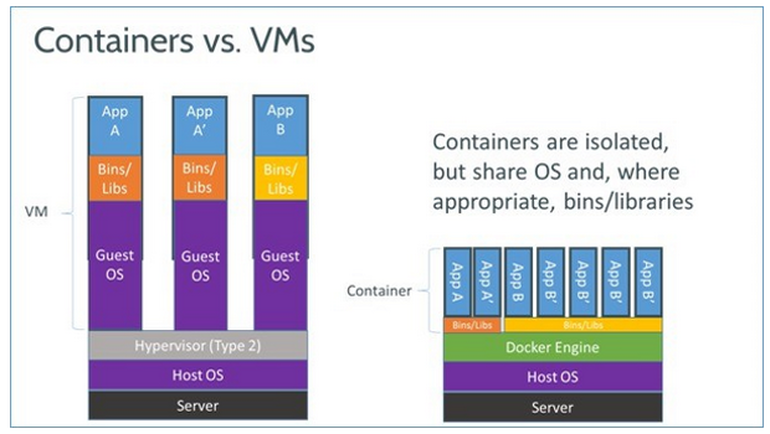
\includegraphics[width=0.8\linewidth]{images/docker-vm-container}
	\caption{Schematischer Vergleich virtuelle Maschine und Container}
	\label{fig:docker}
\end{figure*}

\section{Stand der Implementierungen}
\label{sec_implementations}

\subsection{Verbreitung bei Neuentwicklungen}
asd

\subsection{Verbreitung bei bestehenden Lösungen}
Während Neuentwicklungen 

\subsection{Grenzen von Cloudimplementierungen}
Private Cloud Skalierbarkeit